\documentclass[tikz,border=4pt]{standalone}
\usepackage{pgfplots}
\usepgfplotslibrary{groupplots,statistics}
\pgfplotsset{compat=1.18}

\definecolor{CDr}{HTML}{CC79A7}
\definecolor{CEq}{HTML}{D55E00}
\definecolor{CFl}{HTML}{0072B2}
\definecolor{CTc}{HTML}{56B4E9}
\definecolor{CVo}{HTML}{E69F00}
\definecolor{CWf}{HTML}{009E73}
\definecolor{COrange}{HTML}{E69F00}
\definecolor{CRed}{HTML}{D55E00}
\definecolor{CBlue}{HTML}{0072B2}

\begin{document}
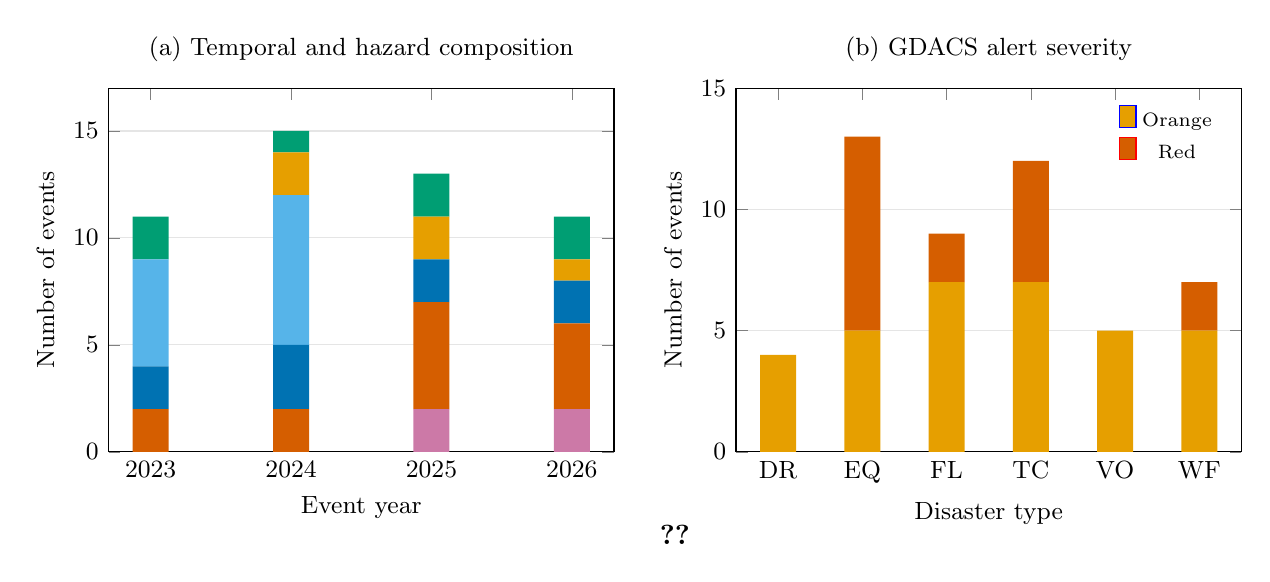
\begin{tikzpicture}
\begin{groupplot}[group style={group size=2 by 1,horizontal sep=1.55cm},
  width=8.0cm,height=6.2cm,tick label style={font=\small},label style={font=\small},
  title style={font=\small},legend style={font=\scriptsize,draw=none,fill=none}]
\nextgroupplot[ybar stacked,bar width=13pt,symbolic x coords={2023,2024,2025,2026},
  xtick=data,ymin=0,ymax=17,ytick distance=5,ymajorgrids,grid style={gray!20},
  xlabel={Event year},ylabel={Number of events},title={(a) Temporal and hazard composition},
  legend columns=3,legend to name=typelegend]
\addplot+[ybar,fill=CDr,draw=none] coordinates {(2023,0) (2024,0) (2025,2) (2026,2)};
\addplot+[ybar,fill=CEq,draw=none] coordinates {(2023,2) (2024,2) (2025,5) (2026,4)};
\addplot+[ybar,fill=CFl,draw=none] coordinates {(2023,2) (2024,3) (2025,2) (2026,2)};
\addplot+[ybar,fill=CTc,draw=none] coordinates {(2023,5) (2024,7) (2025,0) (2026,0)};
\addplot+[ybar,fill=CVo,draw=none] coordinates {(2023,0) (2024,2) (2025,2) (2026,1)};
\addplot+[ybar,fill=CWf,draw=none] coordinates {(2023,2) (2024,1) (2025,2) (2026,2)};
\legend{DR,EQ,FL,TC,VO,WF}
\nextgroupplot[ybar stacked,bar width=13pt,symbolic x coords={DR,EQ,FL,TC,VO,WF},
  xtick=data,ymin=0,ymax=15,ytick distance=5,ymajorgrids,grid style={gray!20},
  xlabel={Disaster type},ylabel={Number of events},title={(b) GDACS alert severity},
  legend pos=north east]
\addplot+[ybar,fill=COrange,draw=none] coordinates {(DR,4) (EQ,5) (FL,7) (TC,7) (VO,5) (WF,5)};
\addplot+[ybar,fill=CRed,draw=none] coordinates {(DR,0) (EQ,8) (FL,2) (TC,5) (VO,0) (WF,2)};
\legend{Orange,Red}
\end{groupplot}
\node at ($(group c1r1.south)!0.5!(group c2r1.south)+(0,-1.05cm)$) {\ref{typelegend}};
\end{tikzpicture}
\end{document}
